\documentclass[11pt]{article}

\usepackage[a4paper]{geometry}
\geometry{left=2.0cm,right=2.0cm,top=2.5cm,bottom=2.5cm}

\usepackage{ctex} % 支持中文的LaTeX宏包
\usepackage{float} % 防止图片乱序
\usepackage{xeCJK} % 中文字体
\usepackage{amsmath,amsfonts,graphicx,subfigure,amssymb,bm,amsthm,mathrsfs,
            mathtools,breqn} % 数学公式和符号的宏包集合
\usepackage{algorithm,algorithmicx} % 算法和伪代码
\usepackage[noend]{algpseudocode} % 算法和伪代码
\usepackage{fancyhdr} % 自定义页眉页脚
\usepackage[framemethod=TikZ]{mdframed} % 创建带边框的框架
\usepackage{fontspec} % 字体设置
\usepackage{adjustbox} % 调整盒子大小
\usepackage{fontsize} % 设置字体大小
\usepackage{tikz,xcolor} % 绘制图形和使用颜色
\usepackage{multicol} % 多栏排版
\usepackage{multirow} % 表格中合并单元格
\usepackage{pdfpages} % 插入PDF文件
\usepackage{listings} % 在文档中插入源代码
\usepackage{lstautogobble} % 去掉源代码多余的空格
\usepackage{xcolor} % 支持彩色
\usepackage{caption} % 支持图片标题
\usepackage{wrapfig} % 文字绕排图片
\usepackage{bigstrut,multirow,rotating} % 支持在表格中使用特殊命令
\usepackage{booktabs} % 创建美观的表格
\usepackage{circuitikz} % 绘制电路图
\usepackage{zhnumber} % 中文序号(用于标题)
\usepackage{tabularx} % 表格折行
\usepackage{enumitem} % 枚举列表
\usetikzlibrary{circuits.ee.IEC} % 使用欧洲风格的电路符号
\usetikzlibrary{circuits.logic.US} % 使用美国风格的逻辑门
\usetikzlibrary{shapes.geometric, arrows.meta, positioning} % 使用流程图的库

% 设置字体
\definecolor{bluekeywords}{rgb}{0.13, 0.13, 1}
\definecolor{greencomments}{rgb}{0, 0.5, 0}
\definecolor{redstrings}{rgb}{0.9, 0, 0}
\definecolor{graynumbers}{rgb}{0.5, 0.5, 0.5}
\lstset{
    autogobble, % 自动移除代码前的空白(对齐代码块)
    columns=fixed, % 使得空格不可拉伸
    showspaces=false, % 不显示空格
    showtabs=false, % 不显示制表符
    breaklines=true, % 自动换行
    showstringspaces=false, % 在字符串中不特别显示空格
    breakatwhitespace=true, % 仅在空白处进行自动换行
    escapeinside={(*@}{@*)}, % 设置一个特殊的标记,允许在代码中插入LaTeX代码
    commentstyle=\color{greencomments}, % 注释的颜色设置为绿色
    keywordstyle=\color{bluekeywords}, % 关键字的颜色设置为蓝色
    stringstyle=\color{redstrings}, % 字符串的颜色设置为红色
    numberstyle=\color{graynumbers}, % 行号的颜色设置为灰色
    identifierstyle=\color{orange}, % 标识符颜色
    basicstyle=\small\ttfamily, % 基本字体样式:小号的等宽字体
    frame=single, % 单线边框
    framesep=12pt, % 边框与代码的间隔
    framerule=0.75pt, % 边框宽度
    xleftmargin=13pt, % 左边距
    xrightmargin=7pt, % 右边距
    tabsize=4, % 制表符宽度
    captionpos=t, % 标题位置在顶部
}
\DeclareCaptionFont{white}{\color{white}}
\DeclareCaptionFormat{listing}{\colorbox[cmyk]{0.43, 0.35, 0.35,0.01}
{\parbox{\textwidth}{\hspace{15pt}#1#2#3}}}
\captionsetup[lstlisting]{format=listing,labelfont=white,textfont=white,
                          singlelinecheck=false, margin=0pt,
                          font={bf,footnotesize}}

\usepackage{hyperref} % 目录,章节,超链接
\hypersetup{
    bookmarks=true,  % 生成书签
    bookmarksnumbered=true  % 书签带章节编号
}

% 轻松引用, 可以用\cref{}指令直接引用, 自动加前缀.
% 例: 图片label为fig:1
% \cref{fig:1} => Figure.1
% \ref{fig:1}  => 1
\usepackage[capitalize]{cleveref}
% \crefname{section}{Sec.}{Secs.}
\Crefname{section}{Section}{Sections}
\Crefname{table}{Table}{Tables}
\crefname{table}{Table.}{Tabs.}

\setCJKmainfont{Source Han Serif CN}
\setmonofont{JetBrains Mono NL}
\punctstyle{kaiming}
% 偏好的几个字体, 可以根据需要自行加入字体ttf文件并调用
% 注意要在自己系统安装字体, 以供调用

\renewcommand{\emph}[1]{\begin{kaishu}#1\end{kaishu}}

% 对 section 等环境的序号使用中文
\renewcommand \thesection{\zhnum{section}、}
\renewcommand \thesubsection{\arabic{subsection}}
\renewcommand \thesubsubsection{\alph{subsubsection}}

%%%%%%%%%%%%%%%%%%%%%%%%%%%
%改这里可以修改实验报告表头的信息
\newcommand{\name}{蓝宇舟}
\newcommand{\studentNum}{2022K8009918005}
\newcommand{\class}{B0911010Y-02}
%%%%%%%%%%%%%%%%%%%%%%%%%%%

\begin{document}

% 标题
\begin{center}
  \LARGE \bf 操作系统第四次作业
\end{center}

\begin{center}
  \emph{姓名} \underline{\makebox[7em][c]{\name}}
  % 如果名字比较长, 可以修改box的长度"8em"为其他值
  \emph{学号} \underline{\makebox[12em][c]{\studentNum}}
  \emph{班级} \underline{\makebox[15em][c]{\class}}\\
\end{center}


% 题目
\begingroup
    \centering
    \LARGE {\bf \Homework} \\[0.5em]
    \large \textbf{姓名:} \Name \hspace{2em}
           \textbf{学号:} \StudentNumber \hspace{2em}
           \textbf{班级:} \Class \par
\endgroup
\rule{\textwidth}{0.4pt}
\printanswers


% 环境说明
\section{环境说明}

\begin{itemize}
    \item 操作系统:{\tt Arch Linux x86_64}
    \item 内核版本:{\tt Linux 6.10.7-zen1-1-zen}
    \item 编译器版本:{\tt gcc (GCC) 14.2.1 20240805}
\end{itemize}


% 测试
\section{测试}

下面分别展示两个系统调用在不同情况下的测试方法。

\subsection{{\tt getpid}}

\subsubsection{测试代码}

\lstinputlisting[language=C, caption={{\tt getpid.c}}]{code/getpid.c}

\subsubsection{说明}

这个测试代码中,我设计了{\tt measure\_glibc} 、 {\tt measure\_syscall}和{\tt measure\_syscall\_inline\_asm}三个函数,分别用于测量{\tt getpid}系统调用的时间:

\begin{enumerate}
    \item {\tt measure\_glibc}使用了{\tt glibc}的{\tt getpid}函数;
    \item {\tt measure\_syscall}使用了{\tt syscall}函数;
    \item {\tt measure\_syscall\_inline\_asm}以内联汇编的方式使用了x86\_64的{\tt syscall}指令。
\end{enumerate}

上述测试分别进行一次,以ns为单位输出测试结果。


\subsection{{\tt open}}

\subsubsection{测试代码}

\lstinputlisting[language=C, caption={{\tt open.c}}]{code/open.c}

\subsubsection{说明}

与{\tt getpid}测试类似,不再赘述。


% 结果及分析
\section{结果及分析}

将这两个测试代码分别编译成可执行文件(使用{\tt -O0}参数),分别运行10次后得到的结果如下图所示:

\begin{figure}[H]
    \centering
    \begin{minipage}[t]{0.45\textwidth}\
        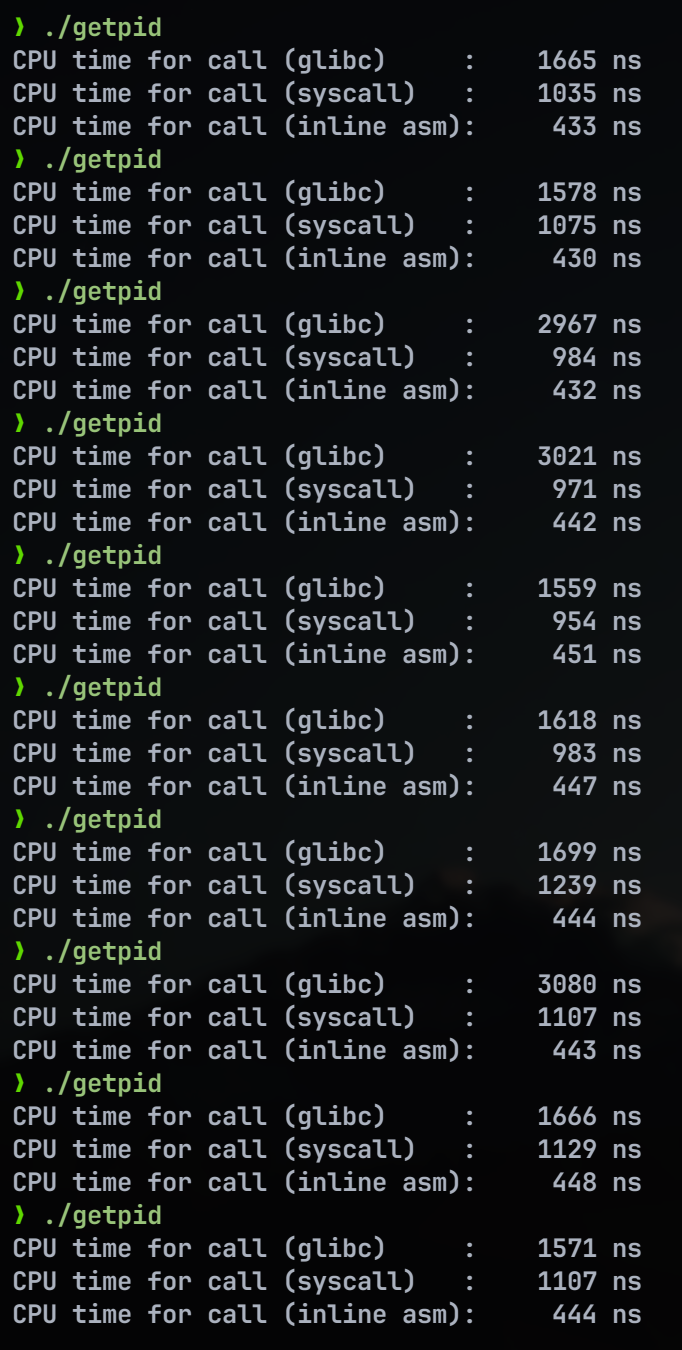
\includegraphics[height=12cm]{fig/getpid.png}
        \caption{{\tt getpid}测试结果}
    \end{minipage}
    \begin{minipage}[t]{0.45\textwidth}\
        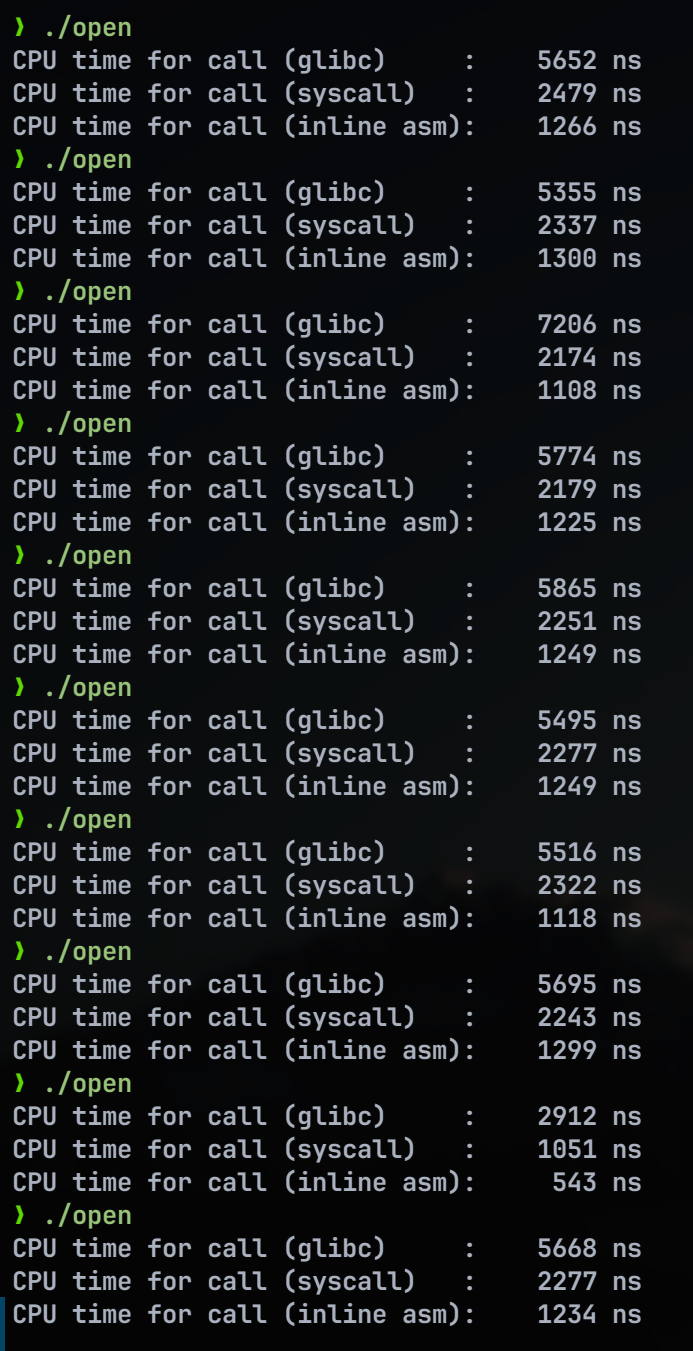
\includegraphics[height=12cm]{fig/open.png}
        \caption{{\tt open}测试结果}
    \end{minipage}
\end{figure}

下面对结果进行分析:

\subsection{同一系统调用在三种不同方法下的时间开销}

\begin{table}[!ht]
    \centering
    \begin{tabular}{|l|l|l|l|}
    \hline
        ~ & glibc & syscall & inline\_asm \\ \hline
        1 & 1665 & 1035 & 433 \\ \hline
        2 & 1578 & 1075 & 430 \\ \hline
        3 & 2967 & 984 & 432 \\ \hline
        4 & 3021 & 971 & 442 \\ \hline
        5 & 1559 & 954 & 451 \\ \hline
        6 & 1618 & 983 & 447 \\ \hline
        7 & 1699 & 1239 & 444 \\ \hline
        8 & 3080 & 1107 & 443 \\ \hline
        9 & 1666 & 1129 & 448 \\ \hline
        10 & 1571 & 1107 & 444 \\ \hline
        average & 2042.4 & 1058.4 & 441.4 \\ \hline
    \end{tabular}
    \hfill
    \begin{tabular}{|l|l|l|l|}
        \hline
            ~ & glibc & syscall & inline\_asm \\ \hline
            1 & 5652 & 2479 & 1266 \\ \hline
            2 & 5355 & 2337 & 1300 \\ \hline
            3 & 7206 & 2174 & 1108 \\ \hline
            4 & 5774 & 2179 & 1225 \\ \hline
            5 & 5865 & 2251 & 1249 \\ \hline
            6 & 5495 & 2277 & 1249 \\ \hline
            7 & 5516 & 2322 & 1118 \\ \hline
            8 & 5695 & 2243 & 1299 \\ \hline
            9 & 2912 & 1051 & 543 \\ \hline
            10 & 5668 & 2277 & 1234 \\ \hline
            average & 5513.8 & 2159 & 1159.1 \\ \hline
        \end{tabular}
    \caption{{\tt getpid}(左)和{\tt open}(右)测试结果}
\end{table}

从以上两个表格可以发现,无论是那种系统调用,每次比对时间开销的结果都是{\tt inline\_asm < syscall < glibc}。这是因为{\tt glibc}对大量系统调用的库,而{\tt syscall}是直接调用系统调用的方法,因此{\tt glibc}的时间开销会更大。相比于{\tt syscall},{\tt inline\_asm}是直接嵌入汇编代码的方法,因此时间开销最小。

显然,封装的越多,函数调用所花费的时间就会越多。个人分析有以下几个原因:

\begin{enumerate}
    \item 函数包装的越复杂,需要执行的指令就会越多,因此时间开销也会更大。
    \item 函数调用涉及到传参,此外更多的函数调用也会涉及到更多的栈操作。以上两者均会增加访问内存的次数。而访存的时间开销是很大的,因此总时间会更长。
\end{enumerate}

\subsection{内联汇编下{\tt getpid}和{\tt open}的时间开销}

\begin{table}[!ht]
    \centering
    \begin{tabular}{|l|l|l|}
    \hline
        ~ & getpid & open \\ \hline
        1 & 433 & 1266 \\ \hline
        2 & 430 & 1300 \\ \hline
        3 & 432 & 1108 \\ \hline
        4 & 442 & 1225 \\ \hline
        5 & 451 & 1249 \\ \hline
        6 & 447 & 1249 \\ \hline
        7 & 444 & 1118 \\ \hline
        8 & 443 & 1299 \\ \hline
        9 & 448 & 543 \\ \hline
        10 & 444 & 1234 \\ \hline
        average & 441.4 & 1159.1 \\ \hline
    \end{tabular}
\end{table}

很显然,{\tt getpid}的时间开销始终小于{\tt open}。

我猜测的原因是{\tt open}则涉及到了文件的打开操作,需要访问磁盘。访问磁盘的时间远远大于访问内存和寄存器的时间,因此{\tt open}的时间开销会更大。

\subsection{其他收获}

本次作业中,我们需要自行编写测试程序来比对不同类型系统调用在不同调用方式下运行花费的时间。在这个过程中,我遇到了一些问题,在尝试攻克的过程也有了不少收获:

最关键的一点,如何正确统计程序执行所花费的时间。起初我测试时,发现同一个测试程序每次运行都会得到不同结果,比如{\tt glibc}花费时间小于其他两个,这与我的分析结论不符合。

结合我对操作系统的粗浅了解,我猜测这与操作系统的调度有关。因为CPU只有一个,所以操作系统会通过快速切换的方式,达到表面上多个程序同时运行的假象。又因为调度的关系,操作系统给不同进程分配的时间未必完全相等。如果我按照现实世界的时间进行测量,势必会受到其他进程的干扰。同时,因为测量对象是系统调用,所以测试样例必须在有{\tt Linux}操作系统的机器上运行,那么在裸机上运行的方法也肯定是行不通的。

此外,和同学探讨过程中也遇到了新的问题:第一次测试时间远多于后面几次。这是因为第一次运行时,动态链接的程序会修改跳转表,他们采用了增加{\tt -static}参数的方法,以静态链接的方式编译程序,从而避免了这个问题。

而我为了解决以上问题,采用了其他方法。想到老师给的提示,即对{\tt gettimeofday}和{\tt clock\_gettime}函数调研。通过查阅资料,我知道了{\tt clock\_gettime}函数可以传入一个{\tt CLOCK\_PROCESS\_CPUTIME\_ID}参数,以直接得到程序运行的CPU时间。这样就不会受其他进程的干扰,也不会受动态链接的影响。

经过测试,我发现这个方法是可行的,得到的结果符合我的分析。这也让我对操作系统的调度有了更深的了解。


\end{document}
